\newpage
\chaptertitle{CHAPTER 3: PROPOSED SYSTEM}
\label{chap:proposed-system}

\subheading{3.1 SYSTEM OVERVIEW}
\label{sec:proposed-overview}

\fontsize{12}{14}\selectfont

NexRag is a local-first academic assistant designed to answer institutional queries through a hybrid evidence pipeline. The system combines three complementary components: a knowledge graph for structured institutional facts, a retrieval engine for unstructured academic documents, and a local language model for grounded response generation. This design is motivated by the observation that academic questions are heterogeneous. Queries such as ``Who teaches Computer Graphics?'' are relational and are best answered from structured data, whereas queries such as ``What are the seminar guidelines?'' depend on narrative explanations embedded in PDF documents.

At runtime, the system accepts a user query through the frontend, forwards it to a FastAPI backend, classifies the query intent, retrieves evidence from the knowledge graph and/or document index, and then constructs a grounded prompt for a local language model served through Ollama. The final response is returned together with supporting evidence, routing mode, and a confidence estimate. The architecture therefore treats answer generation as the final stage of an evidence-selection process rather than as an isolated generative task.

The repository confirms a modular implementation. The API layer coordinates requests, the router performs lightweight intent detection, the graph module executes SPARQL-based retrieval, the retrieval module manages PDF extraction and ranking, and the LLM module produces the final response. The frontend complements this backend pipeline with source inspection, system-status display, and graph-editing support, making the system usable as an operational academic assistant rather than a backend-only prototype.

At a design level, NexRag treats question answering as constrained evidence synthesis. The system does not begin from the assumption that the model already ``knows'' the answer; instead, it treats the model as a formatter and explainer operating over retrieved institutional evidence. This distinction is critical in an educational context because it makes answer quality depend primarily on the correctness of retrieved graph facts and passages rather than on opaque parametric memory. The architecture is therefore intentionally conservative: retrieval and evidence selection occur first, while generation is used to organize and explain already selected content.

\begin{center}
\normalsize \textbf{\textit{Table 3.1: Core Software Stack Used in NexRag}}
\end{center}

\begingroup
\footnotesize
\renewcommand{\arraystretch}{1.12}
\setlength{\tabcolsep}{4pt}
\begin{table}[H]
\centering
\label{tab:software-stack}
\begin{tabularx}{\textwidth}{|>{\RaggedRight\arraybackslash\hspace{0pt}}X|>{\RaggedRight\arraybackslash\hspace{0pt}}X|>{\RaggedRight\arraybackslash\hspace{0pt}}X|}
\hline
\textbf{Layer} & \textbf{Technology} & \textbf{Role} \\ \hline
Frontend & React, Vite, TypeScript & Query input, chat view, sources, status, KG editor \\ \hline
Backend API & FastAPI & Request orchestration and service endpoints \\ \hline
Dense retrieval & Sentence Transformers, FAISS & Embedding generation and vector search \\ \hline
Sparse retrieval & BM25 (\path|rank_bm25|) & Exact-term and lexical search \\ \hline
Reranking & CrossEncoder (\path|ms-marco-MiniLM-L-6-v2|) & Precision ranking of shortlisted chunks \\ \hline
Knowledge graph & RDF/Turtle, Fuseki, SPARQL & Structured institutional fact retrieval \\ \hline
Generation & Ollama, \path|llama3.2:3b| & Local grounded answer generation \\ \hline
\end{tabularx}
\end{table}
\endgroup

\subheading{3.2 SYSTEM ARCHITECTURE}
\label{sec:proposed-architecture}

The architecture follows a layered hybrid-processing model. The frontend collects user questions and displays responses with route and source information. The backend receives the request and invokes a router that categorizes the query into coarse academic intents such as faculty information, course information, regulations, definitions, or general queries. This routing step does not produce the answer by itself; instead, it decides which evidence pathways should be prioritized.

The first evidence pathway is the knowledge graph. When the query is relational or entity-centric, the backend issues SPARQL queries over RDF data stored in Turtle files and served through Apache Jena Fuseki. The second pathway is the document-retrieval engine. Academic PDFs are chunked, indexed, and searched using both dense vector similarity and BM25 lexical ranking. The candidate passages from both paths are reranked and filtered before being passed to the language model. The system can therefore operate in graph mode, vector mode, combined mode, or no-hit mode depending on evidence availability.

\begin{figure}[H]
\centering
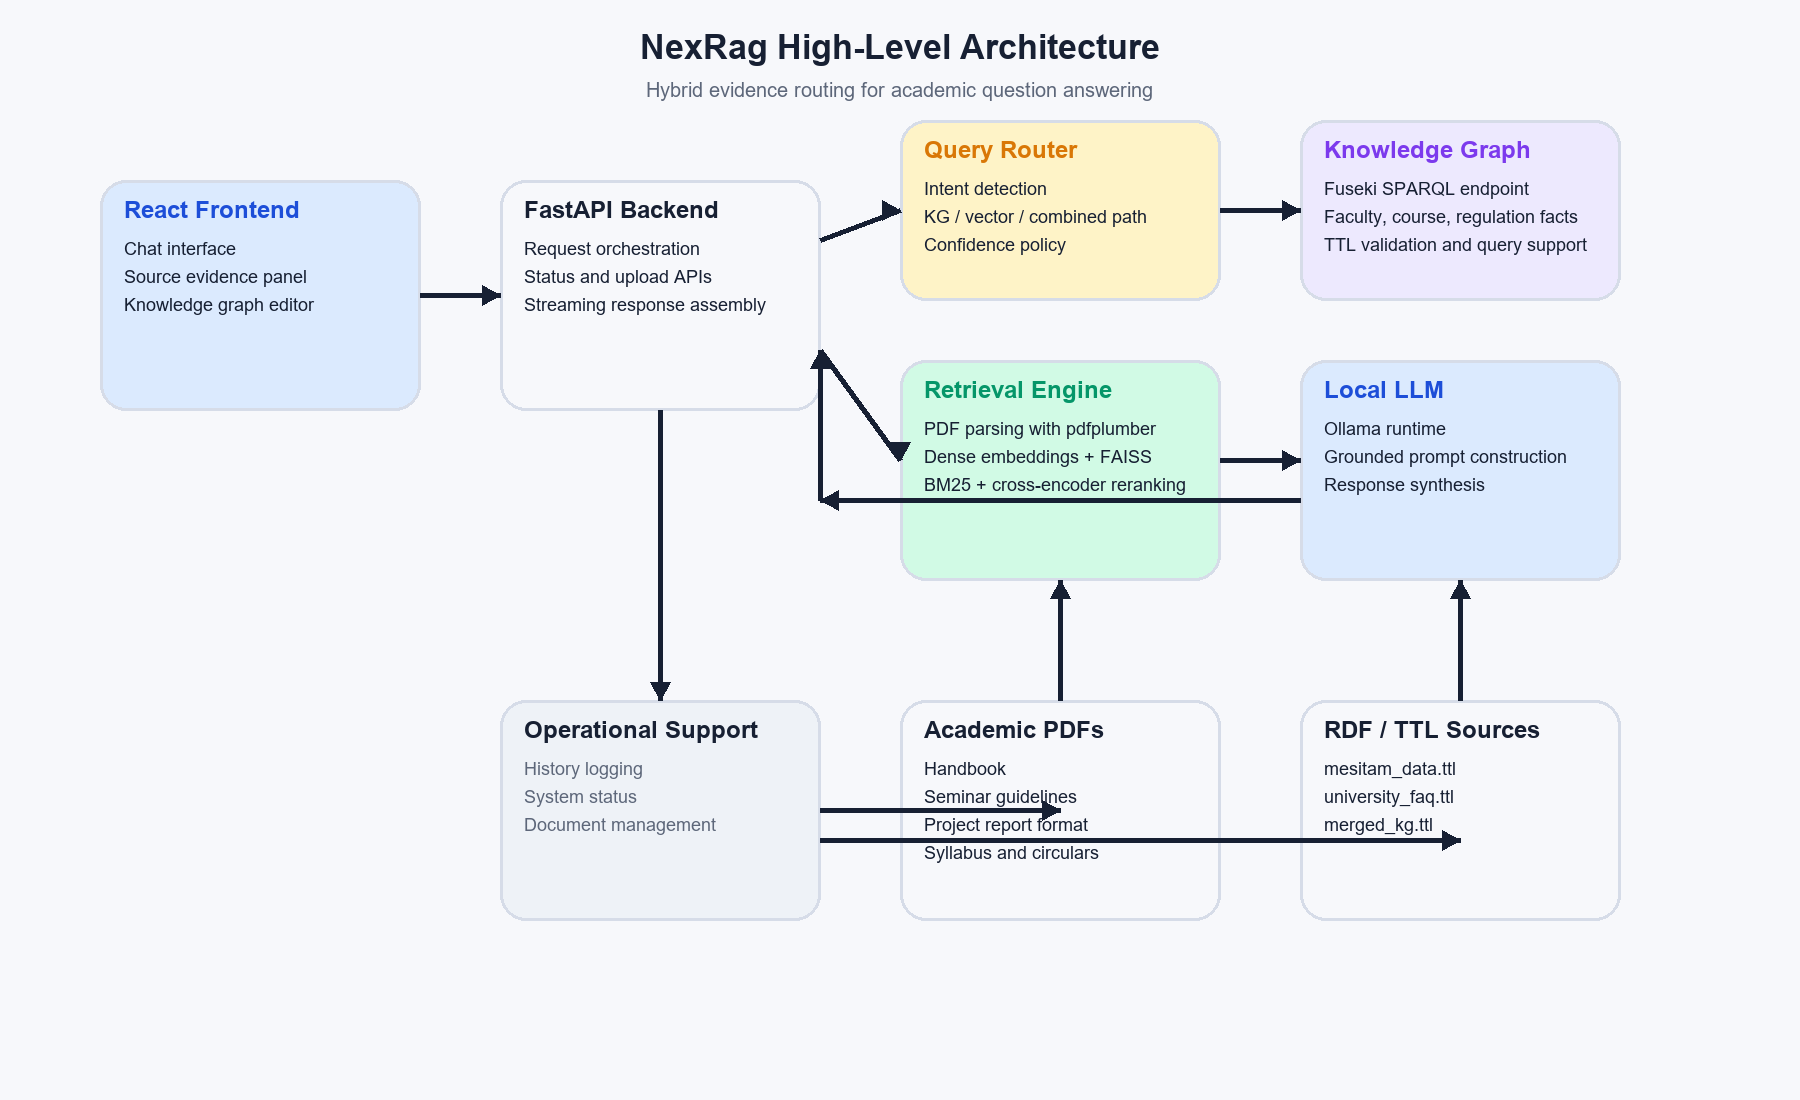
\includegraphics[width=\textwidth]{nexrag_architecture.png}
\label{fig:nexrag-architecture}
\vspace{-0.25cm}
\begin{center}
\normalsize \textbf{\textit{Fig3.1. High-Level Architecture of NexRag}}
\end{center}
\end{figure}

The final step in the architecture is grounded response generation. Retrieved graph facts and top-ranked document snippets are composed into a prompt that instructs the local model to answer from available evidence and avoid unsupported claims. The backend then returns the generated answer, the route label, supporting sources, and a confidence value to the frontend. This architecture improves transparency because users can inspect not only the final answer, but also the evidence path used to produce it.

The architecture also supports controlled degradation. If graph evidence is unavailable, the system can still respond through document retrieval; if retrieval is weak, the user can be shown reduced confidence and limited evidence instead of an artificially certain answer. This behavior is especially important in local deployments, where auxiliary services such as a graph endpoint or model runtime may not always be active simultaneously. By separating routing, retrieval, generation, and status inspection, NexRag remains interpretable even when operating in a reduced-capability state.

\begin{figure}[H]
\centering
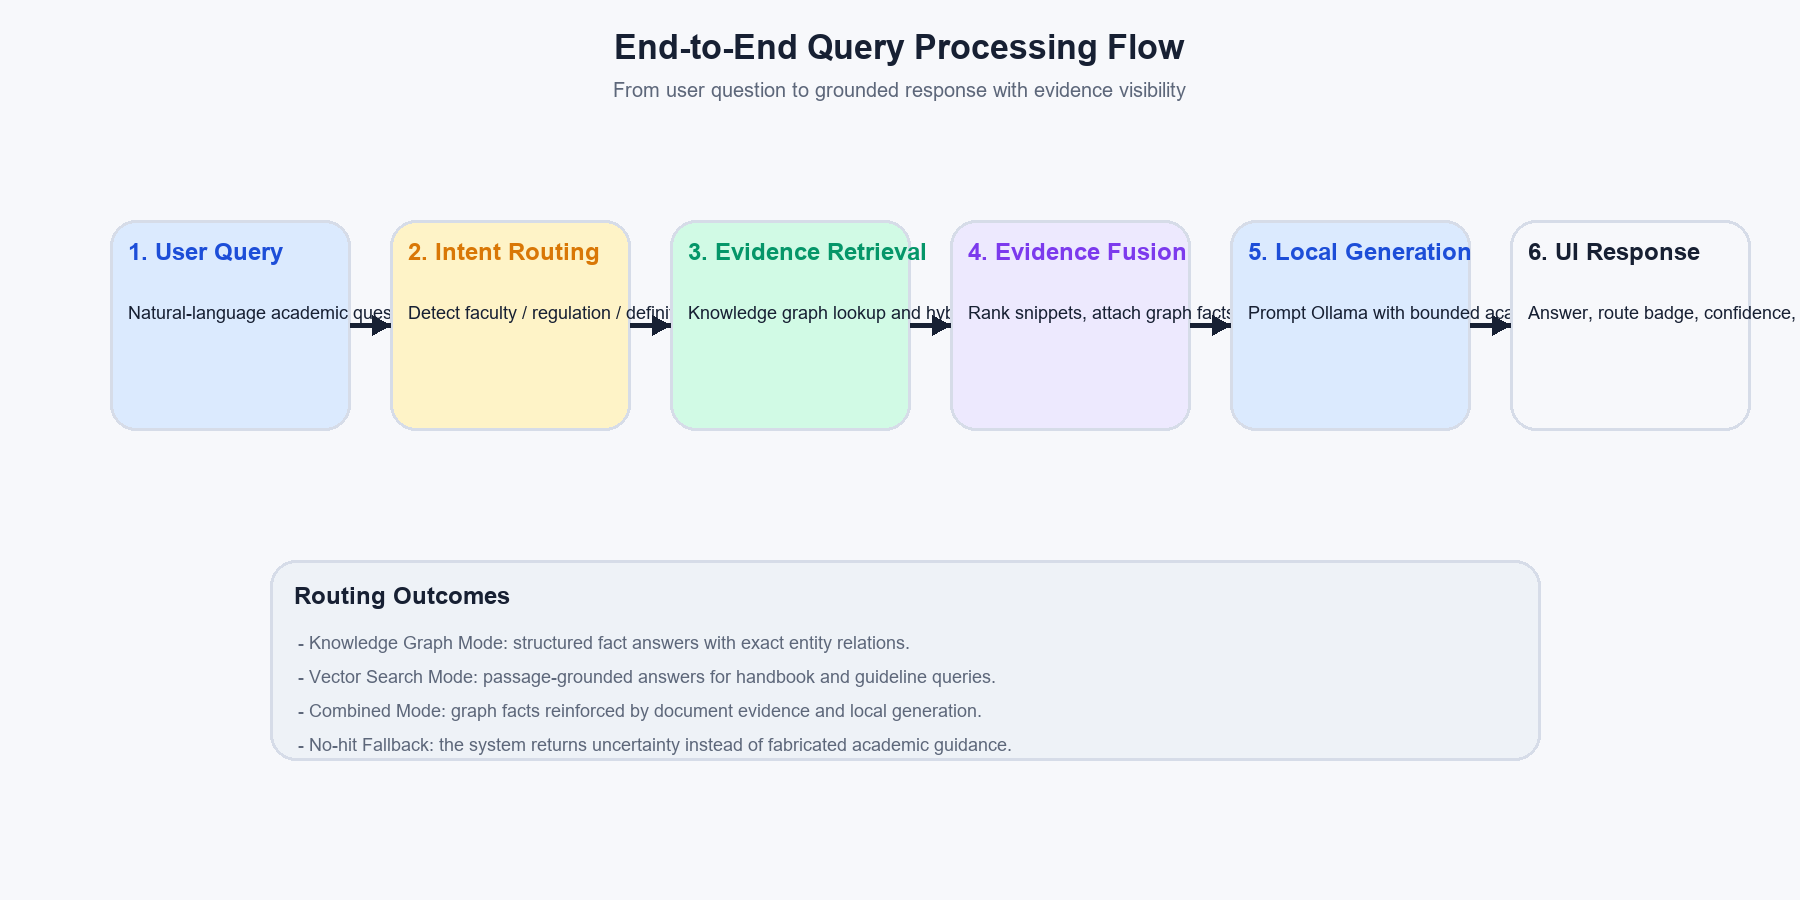
\includegraphics[width=\textwidth]{nexrag_query_flow.png}
\label{fig:nexrag-query-flow}
\vspace{-0.25cm}
\begin{center}
\normalsize \textbf{\textit{Fig3.2. End-to-End Query Processing Flow}}
\end{center}
\end{figure}

\noindent\textbf{3.2.1 ARCHITECTURAL RATIONALE}

The selected architecture is based on complementarity. A graph-only design would provide precise relations but weak explanatory detail, while a document-only design would provide narrative evidence but weaker support for structured entity questions. A generative-only system would remain vulnerable to hallucination. NexRag therefore integrates graph querying, hybrid retrieval, and local generation in a modular manner so that each component addresses a distinct weakness of the others. The modular design also improves maintainability, because routing logic, graph schema, retrieval models, and language-model configuration can evolve independently.

Another reason for this architecture is lifecycle manageability. Institutional documents change periodically, faculty assignments may be revised each semester, and new procedural guidelines may be introduced without notice. A tightly coupled system would make such updates difficult to isolate and validate. The modular architecture avoids that problem by allowing PDF re-indexing, graph updates, and prompt tuning to be performed as bounded maintenance actions. This improves the long-term practicality of the system beyond the initial project demonstration.

\subheading{3.3 MODULES}
\label{sec:proposed-modules}

The implementation is organized into functional modules that coordinate through the API layer. Each module addresses a specific operational responsibility, which makes the system easier to test, extend, and maintain.

\begin{center}
\normalsize \textbf{\textit{Table 3.2: Major Backend Modules and Responsibilities}}
\end{center}

\begingroup
\footnotesize
\renewcommand{\arraystretch}{1.12}
\setlength{\tabcolsep}{4pt}
\begin{table}[H]
\centering
\label{tab:backend-modules}
\begin{tabularx}{\textwidth}{|>{\RaggedRight\arraybackslash\hspace{0pt}}X|>{\RaggedRight\arraybackslash\hspace{0pt}}X|>{\RaggedRight\arraybackslash\hspace{0pt}}X|}
\hline
\textbf{Module} & \textbf{Primary File} & \textbf{Responsibility} \\ \hline
API orchestration & \path|api.py| & Request handling, response assembly, service endpoints \\ \hline
Query routing & \path|router.py| & Coarse intent classification \\ \hline
Knowledge graph service & \path|kg.py| & SPARQL query execution and TTL validation \\ \hline
Retrieval engine & \path|rag.py| & PDF extraction, chunking, indexing, retrieval, reranking \\ \hline
Generation engine & \path|llm.py| & Grounded prompt construction and answer generation \\ \hline
Logging and support & \path|logger.py|, \path|merge_kg.py| & Query history and graph-merge workflows \\ \hline
\end{tabularx}
\end{table}
\endgroup

\noindent\textbf{3.3.1 USER INTERFACE MODULE}

The user interface is implemented with React and Vite and provides three core views: the conversation interface, an intelligence panel, and a knowledge-graph editor. The conversation interface accepts natural-language queries and renders streaming responses with route labels and source summaries. The intelligence panel exposes retrieved documents, graph evidence, model identity, and service readiness. The graph editor allows controlled maintenance of Turtle files through the same interface. This design is important because it transforms the assistant from a hidden pipeline into an explainable and maintainable user-facing system.

\noindent\textbf{3.3.2 API ORCHESTRATION MODULE}

The API module serves as the control layer of the application. It exposes endpoints for status checks, document upload and deletion, chat requests, history retrieval, graph file access, and graph restart workflows. More importantly, it assembles the final chat payload by combining route output, graph evidence, vector evidence, and confidence scoring. Centralizing this logic in \path|api.py| prevents duplication and ensures that the system behaves consistently across standard and streaming chat modes.

\noindent\textbf{3.3.3 QUERY ROUTING MODULE}

The routing module performs lightweight intent classification using keyword-driven heuristics. It identifies categories such as faculty information, course information, regulation, comparison, definition, and general queries. This approach is suitable for a bounded academic domain because common query types are predictable and the rules are easy to maintain. The trade-off is reduced flexibility for ambiguous or highly paraphrased inputs, which is recognized as a future enhancement area.

The router is intentionally coarse-grained rather than over-engineered. Its purpose is not to produce a final semantic label with research-grade accuracy, but to guide the first evidence decision with minimal latency and maximum inspectability. In a bounded academic corpus, this is a practical design choice because many high-frequency questions are repetitive and lexically stable. The router can therefore serve as a lightweight control mechanism while leaving the final relevance decision to retrieval and reranking.

\noindent\textbf{3.3.4 KNOWLEDGE GRAPH MODULE}

The knowledge graph module handles structured institutional facts stored as RDF/Turtle data and queried through SPARQL. It extracts search terms from user queries, matches them to faculty, course, department, or regulation entities, and formats the returned bindings into readable answers. The same module also supports TTL validation and update inspection, warning when an edit removes triples. This makes the graph service both a fact-retrieval subsystem and a controlled data-maintenance layer.

The graph path is particularly important for questions where exact relations matter more than descriptive explanation. Queries about who handles a course, which department offers a subject, or how an entity is connected within the institution benefit from explicit triples rather than paragraph-level similarity. By storing such relations in RDF form, the system separates authoritative institutional facts from less structured descriptive text. This improves explainability because graph answers can be traced back to explicit entities and predicates rather than inferred from loosely related passages.

\noindent\textbf{3.3.5 RETRIEVAL ENGINE MODULE}

The retrieval engine is responsible for processing academic PDFs and producing ranked evidence passages. It extracts text with \path|pdfplumber|, splits text into overlapping chunks, encodes chunks using a sentence-transformer model, stores the vectors in FAISS, and keeps associated metadata for source tracking. At query time it performs both dense retrieval and BM25 search, merges candidate sets, reranks them using a cross-encoder, and filters weak results. This layered design balances semantic recall, lexical precision, and ranking quality.

The chunking and metadata strategy is central to retrieval quality. Each chunk preserves document identity, page-level provenance, and contextual association with neighbouring text so that retrieved evidence remains interpretable when shown to the user. This is necessary because academic rules are often expressed across consecutive clauses, tables, or page sections rather than in isolated sentences. By retaining source metadata throughout the pipeline, NexRag can present answers together with document names, page references, and relevance signals, thereby improving both utility and trust.

\noindent\textbf{3.3.6 LOCAL LANGUAGE MODEL MODULE}

The generation module constructs a grounded prompt that includes the user query, the selected evidence, and instructions to answer conservatively when evidence is insufficient. The system uses a locally served language model through Ollama, which supports privacy-aware and cost-controlled deployment. The generated answer is streamed back to the interface, improving perceived responsiveness without changing the underlying evidence pipeline.

Prompt construction is deliberately evidence-first. Graph facts and document snippets are serialized into a compact context block, and the model is instructed to prefer explicit evidence, avoid unsupported assumptions, and acknowledge insufficiency when necessary. This makes the LLM function as a controlled response synthesizer instead of an unrestricted answer generator. In a college setting, such bounded prompting is preferable because the primary goal is reliability of institutional guidance rather than stylistic elaboration.

\noindent\textbf{3.3.7 LOGGING, HISTORY, AND MAINTENANCE MODULE}

The system also includes operational support components. Query logs are written to a CSV history file, status endpoints expose document and vector-index counts, and the graph workflow supports merge and restart operations. These components do not define the intelligence of the system, but they are essential for maintainability and evaluation because they make runtime behavior inspectable and auditable.

\subheading{3.4 ALGORITHMS USED}
\label{sec:proposed-algorithms}

The intelligence of NexRag depends on a sequence of algorithms rather than a single model. The main computational stages are embedding generation, vector search, lexical ranking, neural reranking, confidence computation, and final evidence-guided generation.

\noindent\textbf{3.4.1 EMBEDDING TECHNIQUE}

The document corpus is divided into chunks and embedded using a sentence-transformer model. If \path|x_i| denotes the \path|i|-th text chunk and \path|f(.)| denotes the embedding model, each chunk vector is computed as:

\manualequation{e_i = f(x_i)}{3.1}

The same encoder is used to generate the query embedding. This representation allows semantically related questions and passages to be compared even when they do not share exact vocabulary. Embedding-based retrieval is therefore valuable for academic queries phrased in natural language rather than formal handbook language.

\noindent\textbf{3.4.2 DENSE VECTOR SEARCH}

FAISS is used for first-stage dense retrieval. Given a query embedding \path|q| and a candidate chunk embedding \path|x|, the current implementation uses Euclidean distance to identify nearby candidates:

\manualequation{d(q, x) = \lVert q - x \rVert_2}{3.2}

Lower distance implies greater similarity in the embedding space. This search is efficient and suitable for first-stage recall, but it is not sufficient by itself because semantically related passages are not always the most authoritative or precise for an institutional query.

\noindent\textbf{3.4.3 COSINE SIMILARITY AS A STANDARD SEMANTIC MEASURE}

Cosine similarity is the standard theoretical measure for comparing embedding direction and is included here because it explains semantic relevance more intuitively:

\manualequation{\cos(q, x) = \frac{q \cdot x}{\lVert q \rVert \lVert x \rVert}}{3.3}

Although the deployed FAISS index uses L2 distance, cosine similarity remains conceptually important because both measures serve the same goal of capturing semantic proximity between a query and candidate passages.

\noindent\textbf{3.4.4 BM25 SPARSE RETRIEVAL}

To preserve lexical precision, NexRag uses BM25 over tokenized chunk text. For a document or chunk \path|D| and query \path|Q|, the BM25 score is:

\manualequation{\begin{aligned} \mathrm{BM25}(D,Q) &= \sum \mathrm{IDF}(q_i)\cdot \\ &\frac{f(q_i,D)(k_1+1)}{f(q_i,D)+k_1\left(1-b+b\frac{|D|}{\mathrm{avgdl}}\right)} \end{aligned}}{3.4}

This stage is particularly useful for exact rule names, course codes, abbreviations, and formal policy phrases. Dense retrieval and BM25 therefore serve different but complementary purposes within the same pipeline.

\noindent\textbf{3.4.5 CROSS-ENCODER RERANKING}

After dense and sparse retrieval, the shortlisted candidates are reranked by a cross-encoder that jointly scores the query and passage. The raw score \path|z| is normalized through a sigmoid function:

\manualequation{\sigma(z) = \frac{1}{1 + e^{-z}}}{3.5}

The normalized value is treated as a relevance score for sorting and thresholding. This stage improves the final quality of the supporting evidence shown to the user.

\noindent\textbf{3.4.6 CONFIDENCE COMPUTATION}

The backend estimates confidence from the available evidence. Graph evidence, vector evidence, and corroboration between the two are combined heuristically into a user-facing percentage. The resulting value is not a calibrated probability, but it provides a practical signal of evidence strength and is preferable to silent overconfidence in an academic assistant.

In operational terms, confidence is better understood as a retrieval-strength indicator than as a probabilistic guarantee of correctness. High confidence implies that the returned answer is supported by strong or corroborating evidence, whereas lower confidence suggests weak retrieval, partial graph support, or marginal ranking scores. This distinction is important because it encourages users to interpret the answer together with its evidence rather than treating the confidence value as a replacement for evidence inspection.

\noindent\textbf{3.4.7 PSEUDO-CODE FOR MAJOR ALGORITHMS}

\textbf{Algorithm 3.1 Document Ingestion and Indexing}

\begin{verbatim}
Input: PDF p, category c
Output: Updated vector and lexical indexes

1. Extract text from p page by page
2. Split text into overlapping chunks
3. Attach metadata: source, page, category
4. Encode chunks into dense vectors
5. Insert vectors into FAISS
6. Rebuild BM25 over chunk texts
7. Persist index and metadata
\end{verbatim}

\textbf{Algorithm 3.2 Hybrid Retrieval and Reranking}

\begin{verbatim}
Input: Query q, top_k
Output: Ranked evidence list

1. Encode q into a dense query vector
2. Retrieve dense candidates from FAISS
3. Score chunks lexically with BM25
4. Merge dense and sparse candidate sets
5. Run cross-encoder on each query-chunk pair
6. Normalize scores and sort in descending order
7. Filter weak candidates and return top_k
\end{verbatim}

\textbf{Algorithm 3.3 Query Routing and Response Assembly}

\begin{verbatim}
Input: User query q
Output: Grounded response payload

1. Classify q using the router
2. Query the knowledge graph if the route suggests it
3. Retrieve ranked document evidence
4. Construct grounded context from available evidence
5. Generate answer using the local LLM
6. Attach route, sources, snippets, and confidence
7. Return payload to the frontend
\end{verbatim}

\noindent\textbf{3.4.8 RRF APPLICABILITY}

Formal Reciprocal Rank Fusion is not implemented in the current repository, but it remains directly applicable. Since NexRag already generates dense and sparse candidate rankings, RRF could be introduced before reranking as an interpretable score-fusion strategy. The present architecture therefore supports future adoption of RRF without redesigning the entire retrieval pipeline.

\subheading{3.5 SYSTEM DESIGN}
\label{sec:proposed-system-design}

The system design of NexRag can be understood through data design, control-flow design, API workflow, and maintenance design. These four views explain how information is stored, how queries are processed, and how the system remains operational over time.

\noindent\textbf{3.5.1 DATA DESIGN}

NexRag uses heterogeneous storage aligned with the nature of the information being handled. Structured institutional facts are stored in RDF/Turtle files and served through Fuseki. Unstructured content remains in PDF form but is mirrored as chunk metadata and dense vectors for retrieval. Query history is written to CSV logs. This design avoids forcing graph facts and document content into the same storage model.

\begin{center}
\normalsize \textbf{\textit{Table 3.3: Conceptual Data Entities and Storage Artefacts}}
\end{center}

\begingroup
\footnotesize
\renewcommand{\arraystretch}{1.12}
\setlength{\tabcolsep}{4pt}
\begin{table}[H]
\centering
\label{tab:data-entities}
\begin{tabularx}{\textwidth}{|>{\RaggedRight\arraybackslash\hspace{0pt}}X|>{\RaggedRight\arraybackslash\hspace{0pt}}X|>{\RaggedRight\arraybackslash\hspace{0pt}}X|}
\hline
\textbf{Information Type} & \textbf{Example Content} & \textbf{Storage Form} \\ \hline
Structured entities & Faculty, departments, courses, regulations & RDF/Turtle files \\ \hline
Graph service data & Merged institutional graph & Fuseki dataset \\ \hline
Document corpus & Handbooks, seminar and report guidelines & Local PDF directory \\ \hline
Dense index & Chunk vectors & \path|vector_store.index| \\ \hline
Chunk metadata & Source, page, text, category & \path|chunks_metadata.pkl| \\ \hline
Interaction history & Question, answer, intent, latency & \path|logs/query_history.csv| \\ \hline
\end{tabularx}
\end{table}
\endgroup

\noindent\textbf{3.5.2 DATA FLOW DESIGN}

The data flow begins with a user query, proceeds through route detection, graph lookup, and/or retrieval, then converges at grounded prompt construction. The answer, along with route and source evidence, is then returned to the user and logged for later analysis. This design makes NexRag a coordination system rather than a single retrieval call.

This flow also supports auditability. Because the route, retrieved evidence, and response metadata are preserved through the backend, the system can later be inspected to determine how a particular answer was produced. Such traceability is valuable in institutional deployments where administrators may need to verify whether an answer reflected graph content, document evidence, or only a weak retrieval fallback.

\begin{figure}[H]
\centering
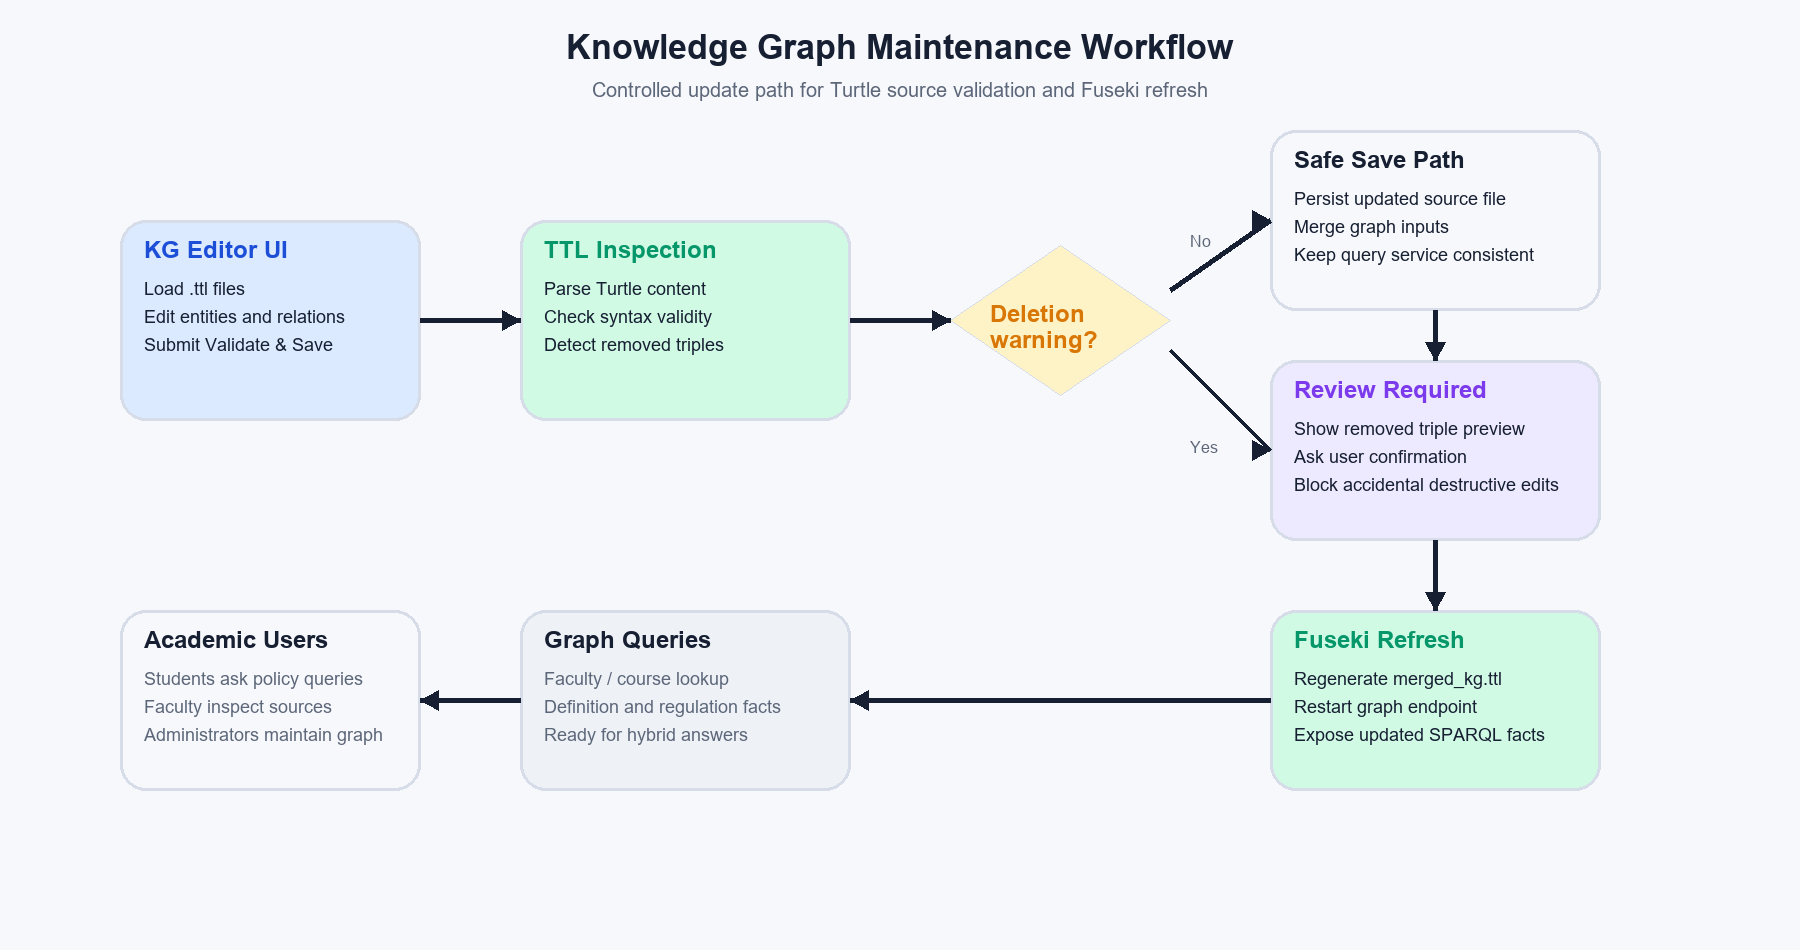
\includegraphics[width=\textwidth]{nexrag_kg_workflow.png}
\label{fig:nexrag-kg-workflow}
\vspace{-0.25cm}
\begin{center}
\normalsize \textbf{\textit{Fig3.3. Knowledge Graph Maintenance and Validation Workflow}}
\end{center}
\end{figure}

\begin{figure}[H]
\centering
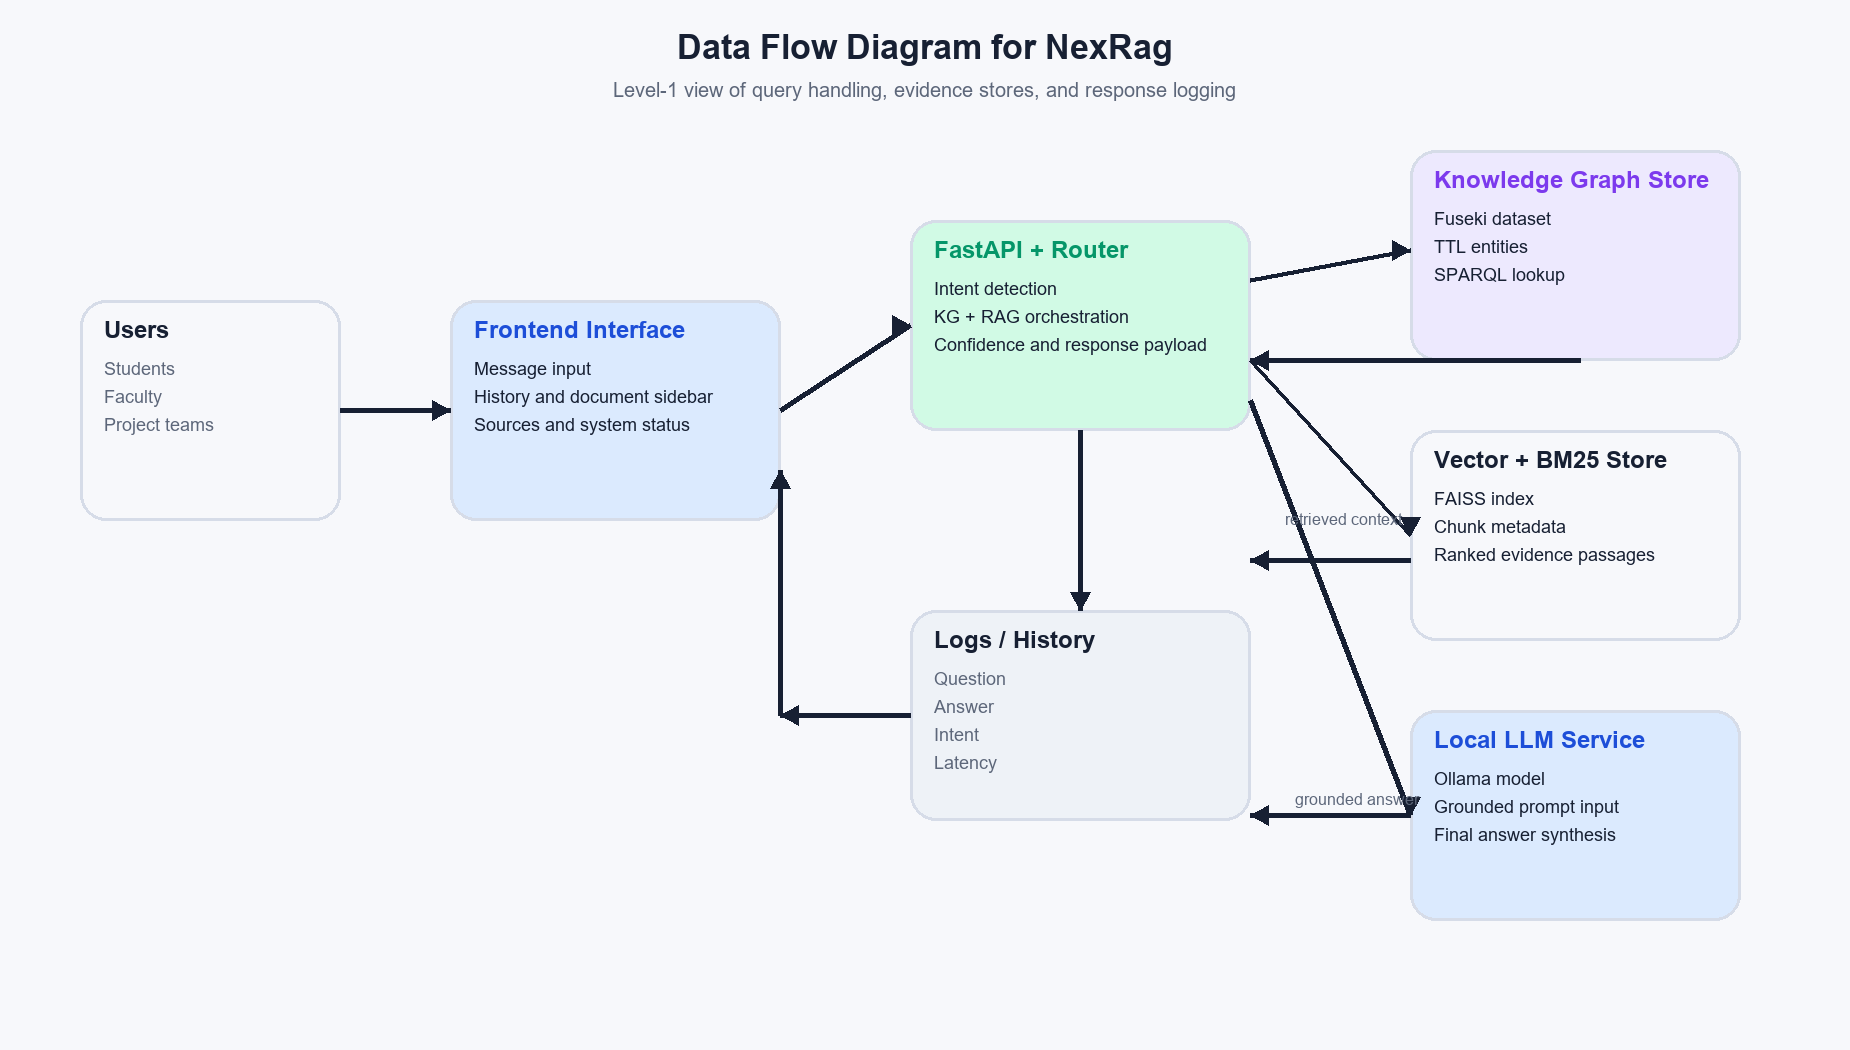
\includegraphics[width=\textwidth]{nexrag_dfd.png}
\label{fig:nexrag-dfd}
\vspace{-0.25cm}
\begin{center}
\normalsize \textbf{\textit{Fig3.4. Data Flow Diagram for the Proposed System}}
\end{center}
\end{figure}

\noindent\textbf{3.5.3 API AND WORKFLOW DESIGN}

The backend exposes endpoints for status checks, document management, chat interaction, history access, graph-source editing, and graph restart. This endpoint structure converts the internal architecture into an operational service model and makes the system easier to verify and maintain.

\begin{center}
\normalsize \textbf{\textit{Table 3.4: API Endpoints and Functional Roles}}
\end{center}

\begingroup
\footnotesize
\renewcommand{\arraystretch}{1.12}
\setlength{\tabcolsep}{4pt}
\begin{table}[H]
\centering
\label{tab:api-endpoints}
\begin{tabularx}{\textwidth}{|>{\RaggedRight\arraybackslash\hspace{0pt}}X|>{\RaggedRight\arraybackslash\hspace{0pt}}X|>{\RaggedRight\arraybackslash\hspace{0pt}}X|}
\hline
\textbf{Endpoint} & \textbf{Method} & \textbf{Function} \\ \hline
\path|/api/status| & GET & Returns PDF, vector, graph, and model status \\ \hline
\path|/api/documents| & GET & Lists indexed PDFs \\ \hline
\path|/api/upload| & POST & Uploads and indexes new documents \\ \hline
\path|/api/documents/{filename}| & DELETE & Removes a document and rebuilds indexes \\ \hline
\path|/api/chat| & POST & Returns complete grounded answer \\ \hline
\path|/api/chat/stream| & POST & Streams grounded answer chunks \\ \hline
\path|/api/history| & GET & Returns recent interaction history \\ \hline
\path|/api/kg-files| & GET & Lists editable Turtle files \\ \hline
\path|/api/kg-source/{filename}| & GET/POST & Reads or updates Turtle source content \\ \hline
\path|/api/kg-save/{filename}| & POST & Validates and saves graph edits \\ \hline
\path|/api/kg-restart| & POST & Merges sources and restarts graph service \\ \hline
\end{tabularx}
\end{table}
\endgroup

The main query workflow is straightforward. A question is submitted from the frontend, routed by intent, checked against the graph when appropriate, searched against the vector and BM25 indexes, reranked, and then passed to the local model together with selected evidence. The system finally returns the answer, the evidence trace, and confidence metadata. This explicit workflow is central to the transparency of the proposed system.

\noindent\textbf{3.5.4 MAINTENANCE DESIGN}

The design also incorporates maintenance as a first-class concern. New PDFs can be uploaded and indexed incrementally. Deleted documents trigger vector-store rebuilding to keep retrieval consistent. Knowledge-graph edits are validated before saving, and potentially destructive graph updates are flagged for inspection. These workflows are necessary because academic knowledge sources are revised over time, and an assistant without maintenance support would quickly lose reliability.

By including these maintenance workflows in the core design, the project recognizes that information systems degrade unless their update path is explicit. The practical value of NexRag therefore depends not only on current retrieval performance, but also on how easily new regulations, revised handbooks, or department-specific graph edits can be incorporated without breaking prior functionality. This systems view is one of the major differences between the proposed work and a narrow proof-of-concept chatbot.

\subheading{3.6 ADVANTAGES}
\label{sec:proposed-advantages}

The proposed system offers several advantages over ordinary chatbots and conventional document search. First, it combines structured and unstructured evidence, allowing both relational and descriptive academic questions to be answered within one framework. Second, it reduces hallucination by grounding generation in graph facts and retrieved passages. Third, it improves user trust by exposing route labels, source snippets, and confidence values rather than returning opaque answers.

The system is also operationally suitable for institutional use. Because it is local-first, it avoids mandatory dependence on external APIs and supports privacy-aware deployment. Its modular implementation allows future upgrades to the router, retriever, graph schema, or language model without redesigning the whole application. The presence of upload, logging, and graph-editing workflows further strengthens its maintainability.

\subheading{3.7 APPLICATIONS}
\label{sec:proposed-applications}

The immediate application of NexRag is institutional academic assistance. Students can use it for attendance rules, seminar and project guidance, faculty-course mapping, and procedural clarifications. Faculty and administrators can use it to reduce repetitive queries and improve the accessibility of official information.

The same architecture is transferable to other bounded domains where structured relations and unstructured documents coexist. Similar systems could support enterprise policy assistance, educational administration, healthcare-training support, or departmental knowledge management. NexRag therefore serves both as a practical institutional tool and as a reusable pattern for local, evidence-aware hybrid assistants.

Within higher education itself, the same design can be extended to multiple administrative layers. Department-level deployments could handle syllabus and faculty information, while institution-level deployments could incorporate examination rules, hostel policies, placement procedures, and accreditation-related knowledge resources. Because the architecture already separates graph facts, document retrieval, and generation, such expansion mainly requires corpus growth and schema extension rather than a complete redesign. This makes NexRag a scalable architectural pattern even if the present implementation remains intentionally bounded.
